% How far a translation gets, by complexity bucket - run 20260904-190539.
% Generated by evaluation/figures/pipeline_funnel.py - do not edit by hand.
%
% Requires, in the document preamble:
%   \usepackage{pgfplots}
%   \pgfplotsset{compat=1.18}
%
% Then: % How far a translation gets, by complexity bucket - run 20260904-190539.
% Generated by evaluation/figures/pipeline_funnel.py - do not edit by hand.
%
% Requires, in the document preamble:
%   \usepackage{pgfplots}
%   \pgfplotsset{compat=1.18}
%
% Then: % How far a translation gets, by complexity bucket - run 20260904-190539.
% Generated by evaluation/figures/pipeline_funnel.py - do not edit by hand.
%
% Requires, in the document preamble:
%   \usepackage{pgfplots}
%   \pgfplotsset{compat=1.18}
%
% Then: % How far a translation gets, by complexity bucket - run 20260904-190539.
% Generated by evaluation/figures/pipeline_funnel.py - do not edit by hand.
%
% Requires, in the document preamble:
%   \usepackage{pgfplots}
%   \pgfplotsset{compat=1.18}
%
% Then: \input{figures/pipeline-funnel-20260904-190539.tex}
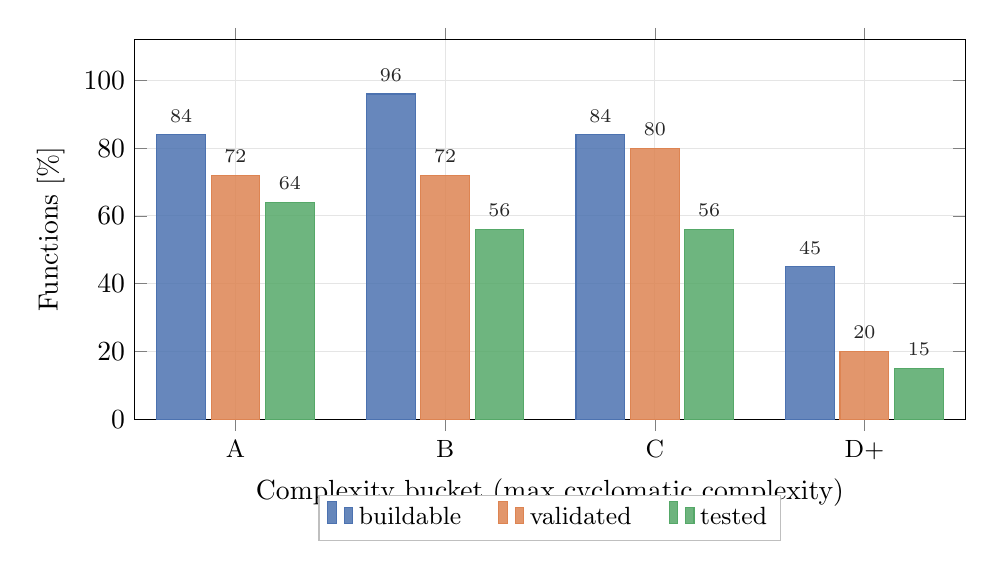
\begin{tikzpicture}
\definecolor{buildable}{HTML}{4c72b0}
\definecolor{validated}{HTML}{dd8452}
\definecolor{tested}{HTML}{55a868}
\begin{axis}[
  ybar,
  width=\linewidth, height=6.4cm,
  bar width=0.62cm,
  enlarge x limits=0.16,
  ymin=0, ymax=112,
  ytick={0,20,40,60,80,100},
  ylabel={Functions [\%]},
  xlabel={Complexity bucket (max cyclomatic complexity)},
  symbolic x coords={A,B,C,Dplus},
  xtick=data, xticklabels={A,B,C,D+},
  x tick label style={font=\small},
  grid=major, grid style={draw=black!10},
  nodes near coords,
  nodes near coords style={font=\scriptsize, /pgf/number format/precision=0,
                           /pgf/number format/fixed, /pgf/number format/fixed zerofill=false},
  every node near coord/.append style={yshift=1pt},
  legend style={at={(0.5,-0.20)}, anchor=north, legend columns=3,
                draw=black!25, font=\small, /tikz/every even column/.append style={column sep=0.4cm}},
]
\addplot[draw=buildable, fill=buildable, fill opacity=0.85] coordinates {(A,84.0) (B,96.0) (C,84.0) (Dplus,45.0)};
\addplot[draw=validated, fill=validated, fill opacity=0.85] coordinates {(A,72.0) (B,72.0) (C,80.0) (Dplus,20.0)};
\addplot[draw=tested,    fill=tested,    fill opacity=0.85] coordinates {(A,64.0) (B,56.0) (C,56.0) (Dplus,15.0)};
\legend{buildable, validated, tested}
\end{axis}
\end{tikzpicture}

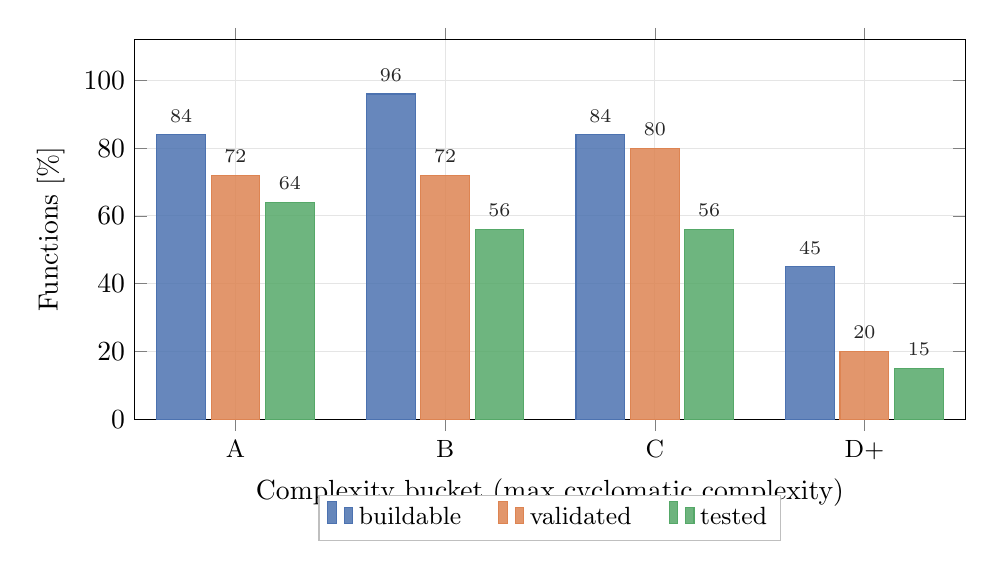
\begin{tikzpicture}
\definecolor{buildable}{HTML}{4c72b0}
\definecolor{validated}{HTML}{dd8452}
\definecolor{tested}{HTML}{55a868}
\begin{axis}[
  ybar,
  width=\linewidth, height=6.4cm,
  bar width=0.62cm,
  enlarge x limits=0.16,
  ymin=0, ymax=112,
  ytick={0,20,40,60,80,100},
  ylabel={Functions [\%]},
  xlabel={Complexity bucket (max cyclomatic complexity)},
  symbolic x coords={A,B,C,Dplus},
  xtick=data, xticklabels={A,B,C,D+},
  x tick label style={font=\small},
  grid=major, grid style={draw=black!10},
  nodes near coords,
  nodes near coords style={font=\scriptsize, /pgf/number format/precision=0,
                           /pgf/number format/fixed, /pgf/number format/fixed zerofill=false},
  every node near coord/.append style={yshift=1pt},
  legend style={at={(0.5,-0.20)}, anchor=north, legend columns=3,
                draw=black!25, font=\small, /tikz/every even column/.append style={column sep=0.4cm}},
]
\addplot[draw=buildable, fill=buildable, fill opacity=0.85] coordinates {(A,84.0) (B,96.0) (C,84.0) (Dplus,45.0)};
\addplot[draw=validated, fill=validated, fill opacity=0.85] coordinates {(A,72.0) (B,72.0) (C,80.0) (Dplus,20.0)};
\addplot[draw=tested,    fill=tested,    fill opacity=0.85] coordinates {(A,64.0) (B,56.0) (C,56.0) (Dplus,15.0)};
\legend{buildable, validated, tested}
\end{axis}
\end{tikzpicture}

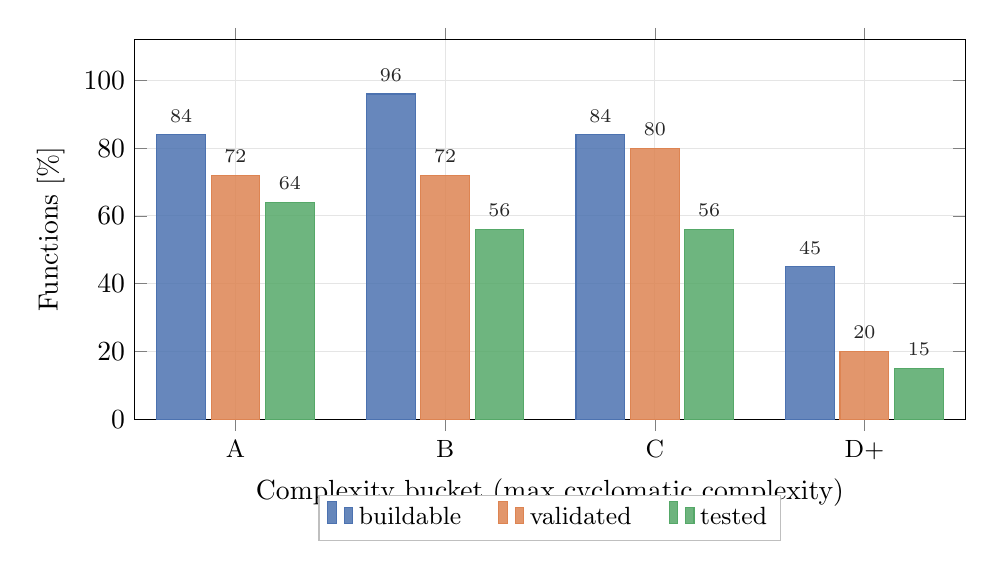
\begin{tikzpicture}
\definecolor{buildable}{HTML}{4c72b0}
\definecolor{validated}{HTML}{dd8452}
\definecolor{tested}{HTML}{55a868}
\begin{axis}[
  ybar,
  width=\linewidth, height=6.4cm,
  bar width=0.62cm,
  enlarge x limits=0.16,
  ymin=0, ymax=112,
  ytick={0,20,40,60,80,100},
  ylabel={Functions [\%]},
  xlabel={Complexity bucket (max cyclomatic complexity)},
  symbolic x coords={A,B,C,Dplus},
  xtick=data, xticklabels={A,B,C,D+},
  x tick label style={font=\small},
  grid=major, grid style={draw=black!10},
  nodes near coords,
  nodes near coords style={font=\scriptsize, /pgf/number format/precision=0,
                           /pgf/number format/fixed, /pgf/number format/fixed zerofill=false},
  every node near coord/.append style={yshift=1pt},
  legend style={at={(0.5,-0.20)}, anchor=north, legend columns=3,
                draw=black!25, font=\small, /tikz/every even column/.append style={column sep=0.4cm}},
]
\addplot[draw=buildable, fill=buildable, fill opacity=0.85] coordinates {(A,84.0) (B,96.0) (C,84.0) (Dplus,45.0)};
\addplot[draw=validated, fill=validated, fill opacity=0.85] coordinates {(A,72.0) (B,72.0) (C,80.0) (Dplus,20.0)};
\addplot[draw=tested,    fill=tested,    fill opacity=0.85] coordinates {(A,64.0) (B,56.0) (C,56.0) (Dplus,15.0)};
\legend{buildable, validated, tested}
\end{axis}
\end{tikzpicture}

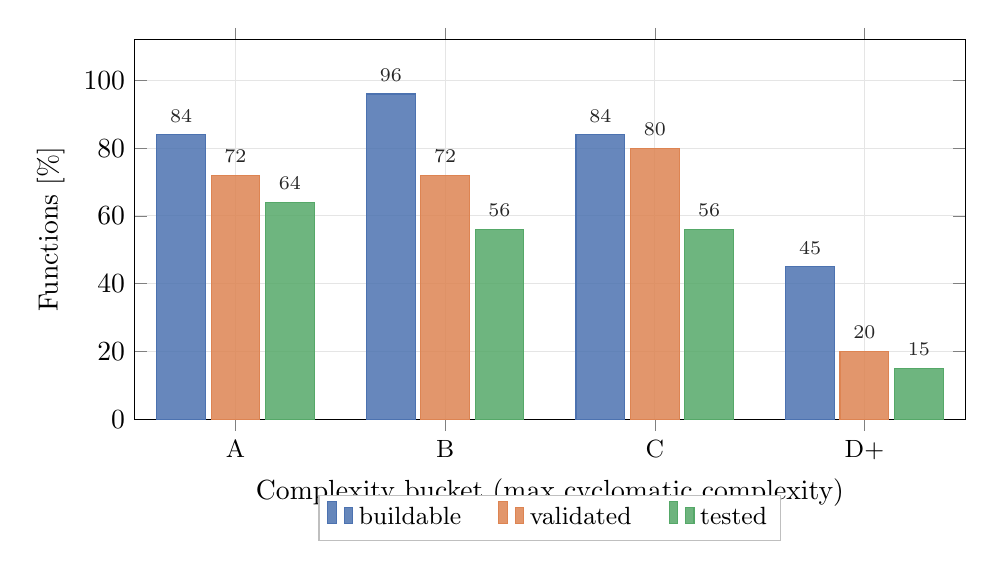
\begin{tikzpicture}
\definecolor{buildable}{HTML}{4c72b0}
\definecolor{validated}{HTML}{dd8452}
\definecolor{tested}{HTML}{55a868}
\begin{axis}[
  ybar,
  width=\linewidth, height=6.4cm,
  bar width=0.62cm,
  enlarge x limits=0.16,
  ymin=0, ymax=112,
  ytick={0,20,40,60,80,100},
  ylabel={Functions [\%]},
  xlabel={Complexity bucket (max cyclomatic complexity)},
  symbolic x coords={A,B,C,Dplus},
  xtick=data, xticklabels={A,B,C,D+},
  x tick label style={font=\small},
  grid=major, grid style={draw=black!10},
  nodes near coords,
  nodes near coords style={font=\scriptsize, /pgf/number format/precision=0,
                           /pgf/number format/fixed, /pgf/number format/fixed zerofill=false},
  every node near coord/.append style={yshift=1pt},
  legend style={at={(0.5,-0.20)}, anchor=north, legend columns=3,
                draw=black!25, font=\small, /tikz/every even column/.append style={column sep=0.4cm}},
]
\addplot[draw=buildable, fill=buildable, fill opacity=0.85] coordinates {(A,84.0) (B,96.0) (C,84.0) (Dplus,45.0)};
\addplot[draw=validated, fill=validated, fill opacity=0.85] coordinates {(A,72.0) (B,72.0) (C,80.0) (Dplus,20.0)};
\addplot[draw=tested,    fill=tested,    fill opacity=0.85] coordinates {(A,64.0) (B,56.0) (C,56.0) (Dplus,15.0)};
\legend{buildable, validated, tested}
\end{axis}
\end{tikzpicture}
